
\section{Multi Agent Research And Simulation}
        \label{section:MARS}
        The MARS Group is a simulation framework developed 
        in HAW Hamburg as a  part of the student research project. The project can be classified as a
        Distributed System \cite{DistributedSystems} designed to carry out simulations of a given model 
        \cite{HAWHamburgMARS}. 
        A model describes a digital prototype of a physical agents i.e wolves, sheep, grass etc 
        which can be simulated to predict a real world scenario. A simple model would
        be the wolves and sheep, using this prototype one can simulate the interaction between the agents. 
        As a result one can analyze the population change between them for this model. Also, Agent-Based Traffic
        models have been developed, which simulates realistic traffic situations in a city scale with great accuracy 
        using the MARS framework \cite{TrafficModel}.

        \par
        \subsection{MARS Resource Hierarchy}
        \label{subsection:MARSResource}
        To leverage the MARS framework in executing a simulation, specific steps that have to be 
        carried out in a chronological manner. The order in which the resources are created have to follow a specific sequence, which is
        the MARS Resource Hierarchy. 
        \begin{enumerate}
            \item 
                \textbf{Create a project}: A project can be defined as a collection of all the resources
                and the simulation results. The resources include models,  scenario description, result configurations, simulation plans,
                simulation runs, simulation results and different files required by the model
                like GIS\footnote{\label{footnote:GIS}GIS: Geographic Information System} Layers \cite[p.~1]{{GIS}}
                Time series \cite{Timeseries} layer etc.
            \item
                \textbf{Upload models and corresponding files}:  The model upload is the first step required
                for a simulation to take place. The model contains information about how the agents behave
                during a simulation run. A model can also be dependent upon other files such as 
                GIS Layers \cite[p.~1]{{GIS}} , Time series \cite{Timeseries} Layer etc, where they are 
                uploaded separately. 

            \item 
                \textbf{Create a scenario}: A scenario of a project can be described as the initialization of the model.
                In process of creating a scenario, attributes like number of agents i.e. wolves, sheep are specified, 
                the uploaded layers like the GIS, Time series etc, if required, are assigned to the model. Also,
                the execution duration parameters of the simulation run are configured.

            \item 
                \textbf{Configure result configuration}: The result configuration enables the user to choose
                the agents desired to be executed in the simulation. This means in the result 
                configuration, one can turn off the 'wolves' output in the Wolves and Sheep models.
            \item  
                \textbf{Create simulation plan and run}: A simulation plan is a complete description of the
                 simulation which includes, scenario and result configuration. For the execution of a simulation
                 one must run the simulation plan, which creates
                 a simulation run. A simulation run contains all the metadata i.e. simulation id, simulation 
                 job status i.e. running, failed, creating etc. Using the simulation run one can analyze the 
                 simulation results.
        \end{enumerate} 
        
        \begin{figure}[H]
            \centering 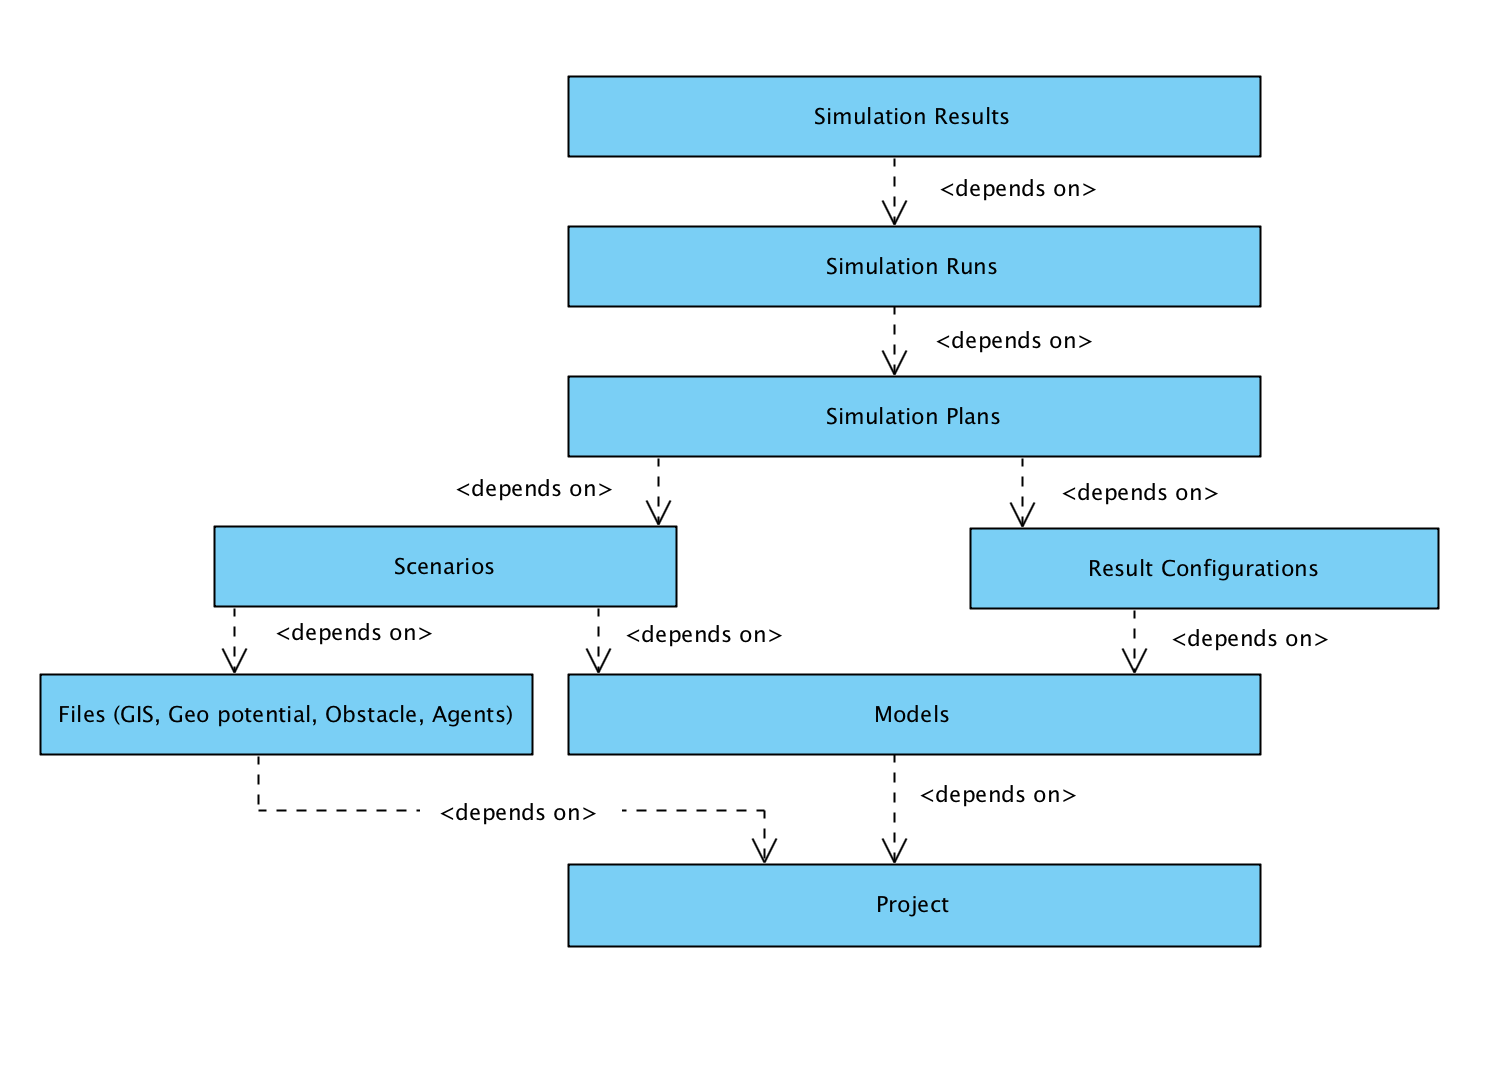
\includegraphics[scale=0.6]{grafiken/marsDependency.png}
            \caption{MARS Resource UML dependency graph \cite{DepDiagram}}
            \label{fig:marsDependency}
        \end{figure}
        
        Figure \ref{fig:marsDependency} shows how the MARS\footnote{MARS: Multi Agent Research and Simulation} 
        resources are dependent. It can be observed
        that the order of existence of the resources have to be from the project to the simulation results 
        (bottom to top) when adding a new simulation. Failure to follow this graph will result in failure to
        successfully run a simulation.

        \begin{figure}[H]
            \centering 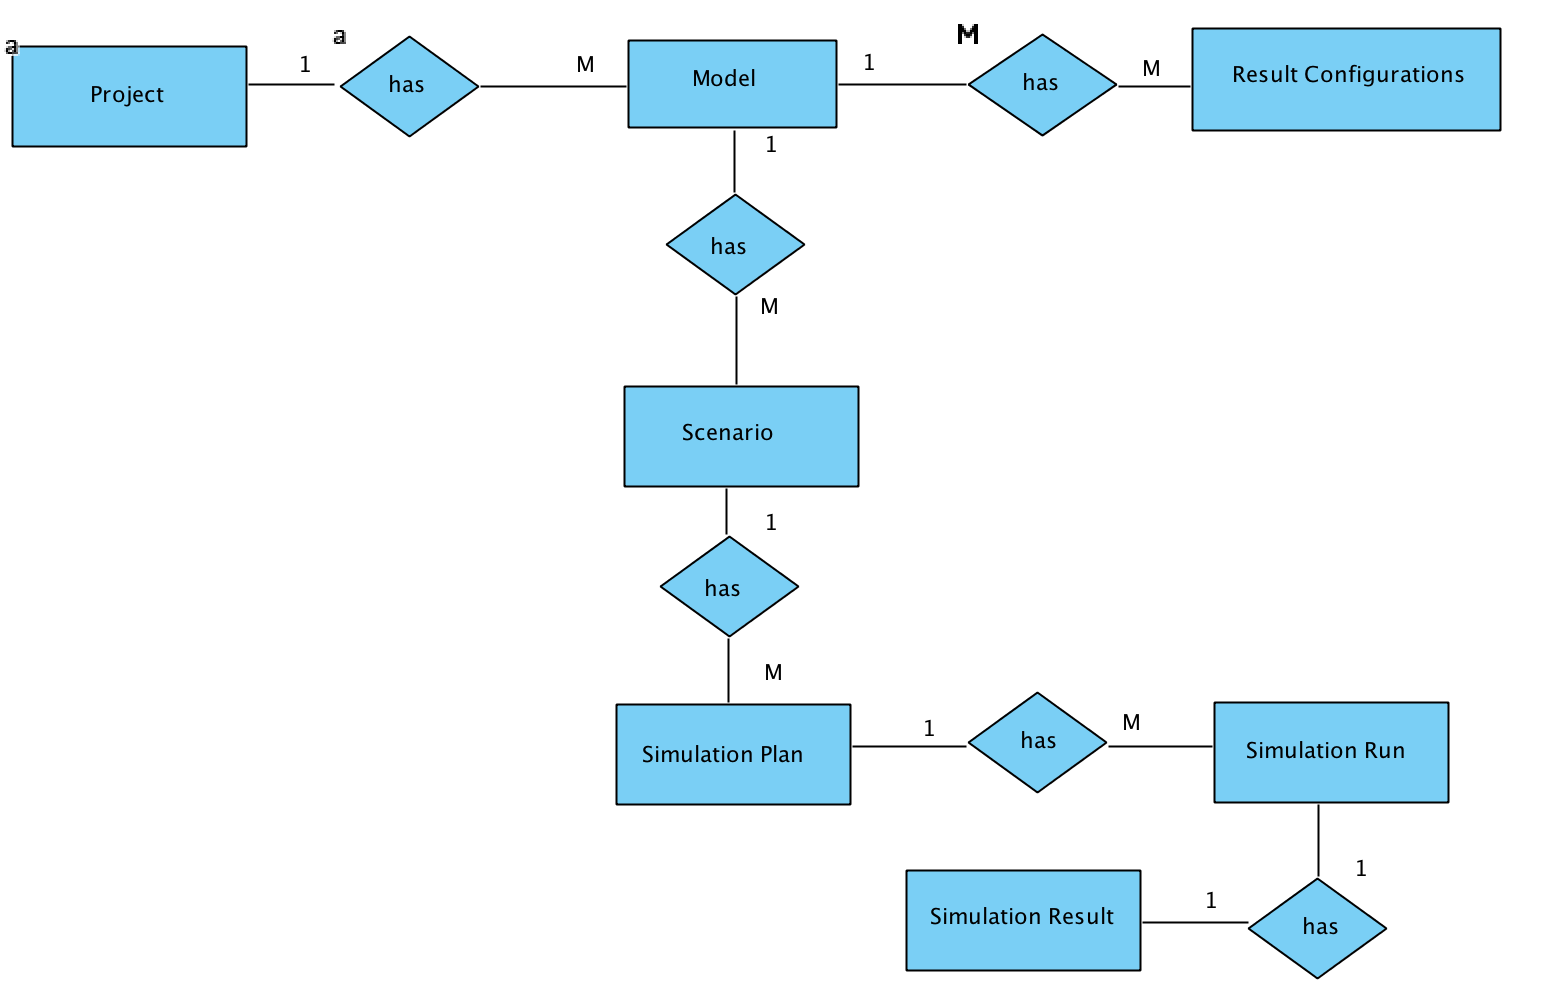
\includegraphics[scale=0.6]{grafiken/ERMars.png}
            \caption{Chen notation Entity Relation Diagram for MARS resources}
            \label{fig:ERMars}
        \end{figure}
        
        Figure \ref{fig:ERMars} intends to show the data flow of the MARS Resources. From this figure it becomes obvious 
        how the resources are dependent upon each other. This follows the hierarchal structure seen in Figure \ref{fig:marsDependency},
        where the project data is at the top and no other entity can persist without it. A pattern for the cardinality of the entities can be observed.
        The lower level entity can only have a reference to one of its parent entity, where as the parent can have multiple children. An exception to this
        pattern is between Simulation Run and Simulation results. A Simulation run may not have multiple results because it represents a job which will produce
        the output i.e. Simulation Results. It is also to be mentioned that every entity expect the project is identified as a weak entity because they cease not 
        to exist without its parent entity. 

        Furthermore, the different data flow mentioned in Figure \ref{fig:ERMars} are handled by various services in the MARS framework. 
        Table \ref{table:MARS Resource Hierarchy Service Overview} gives an overview of the elementary services which are responsible for 
        creating and running simulations.For simplicity reason, only the services
        which has direct dependency with Archive service is mentioned.
        \begin{table}[h!]
            \centering
            \begin{tabular}{|p{4cm}|p{11cm}|}
                \hline
                    \textbf{Service Name}  & \textbf{Description}\\
                \hline
                    Project Service & 
                    Handles Project resources. \\
                \hline
                    File Service
                    & Handles the import and export of different File resources i.e. models, GIS\footnote{\label{footnote:GIS}GIS: Geographic Information System}, 
                    Time series etc.\\
                \hline
                    Metadata Service  & Manages all the Metadata resources.\\
                \hline
                    Resultcfg Service  & The Result configurations which holds the mapping of the models are handled.\\
                \hline
                    Scenario Service  & The Scenario resources management is handled with this service.\\
                \hline
                    Sim-runner Service  & Handles Simulation plans and Simulation run .\\
                \hline
            \end{tabular}
            \caption{MARS Resource Hierarchy Elementary Services Overview}
            \label{table:MARS Resource Hierarchy Service Overview}     
        \end{table}    